\chapter{System Identification: $\ell_p$-norm estimators}

We have introduced in the first chapter the concept of \textit{System Identification} and we caught the importance of experimentally collected data, clearly in this more or less complex procedure one has to take into account that since that -- the data are collected by performing experiments on the real plant, they can be affected by \textbf{uncertainty/measurement noise}.\\
Moreover, even if the system to be identified  is a \textbf{continuous-time one} the most natural model for SysId is the discrete-time one, since samples of continuos time signals are collected.

\section{Regression form for describing dynamical systems}
There are evidences that -- in a quite general manner -- any dynamical system can be represented by using the so-called \textbf{regression form}, which stabilizes a relation between the current output, the input samples and the samples of the previous output. It is defined as follows:
\begin{equation}    \label{eq:reg_form}
    y(k)=f(y(k-1), y(k-2),  ..., y(k-n), u(k-1), ..., u(k-m), \theta)
\end{equation}
For any physical system $m\le{n}$ where $n$ is the system order that is the number of \textit{state variables}.

\section{Error-in-variables(EIV): General setting for SysId}
The most general setting describing an experiment performed on a plant to be identified is the \textbf{Error-in-variables (EIV)}, here both output $y(k)$ and input $u(k)$ are affected by measurement noise $\eta(k)$ and $\xi(k)$ respectively. Then the collected data can be represented by:
\begin{align} 
    &\tilde{u}(k) = u(k) + \xi(k)\\
    &\tilde{y}(k) = y(k) + \eta(k)
\end{align} 
In some situation the sequence input $u(k)$ can be assumed to be perfectly known so $\xi(k)=0$, because we build it in order to stimulate the system.\footnote{
    Later, when the concept on noise will be better formalized, we will give to such an approach the name of \textbf{output error (OE)}.
}
However, the \textbf{EIV} is more general and encapsulate also the situation in which the system to be identified is a subsystem from a more complex plant, then, since both $u(t)$ and $y(t)$ must be measured, both input and output are corrupted  by uncertainty/measurement noise. 

The following is a figure that shows schematically the setting we have just described: 

\begin{figure}[h]
    \centering
    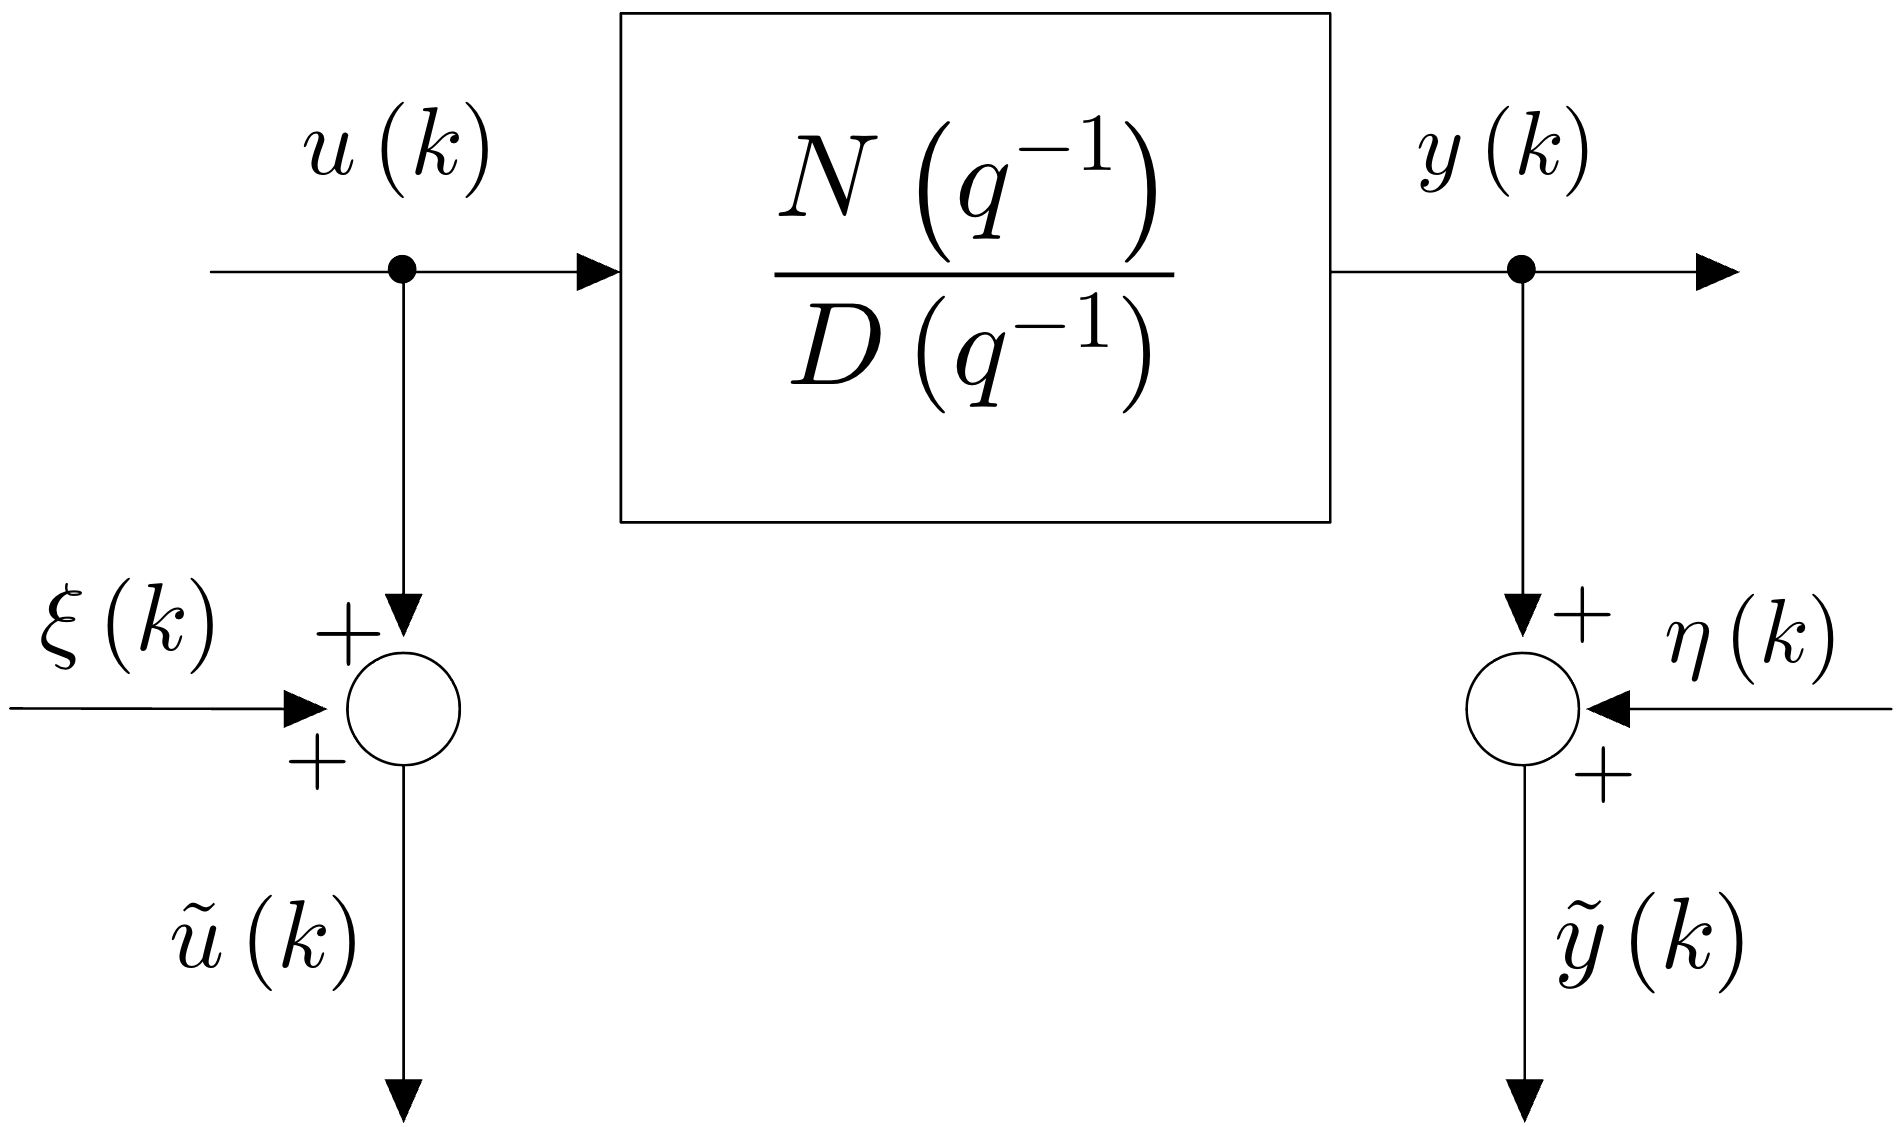
\includegraphics[scale=0.15]{img/EIV.jpeg}
    \caption{EIV SysId setting}
\end{figure}

\vspace{0.5cm}
\noindent
Once we have fixed the setting, the a-priori information to provide are about: 
\begin{itemize}
    \item The \textbf{model} for example $f\in\mathcal{F}$ where $\mathcal{F}$ is associated with a certain class of systems (eg. LTI, nonlinear, stable...)
    \item The \textbf{noise} and in particular information reguarding the \textbf{statistical distribution} (white, gaussian...) or the \textbf{boundedness} (depending on the approach we are going to follow).
\end{itemize}

\noindent
Now we are going to show an example which helps us to understand why the \textit{regression form} is an effective model for describing in the most general manner a dynamical system. 

\subsubsection{Example (Regression form for a second order LTI system)}
Let us consider a case in which we want to derive a model for a linear time-invariant system of the second order (a-priori assumption on the model: $f\in\mathcal{LTI}$, $n=2$), furthermore suppose there is no noise in the data. The regression form $y(u(k),\theta)$ is:
\begin{equation}\label{eq:reg_form}
    \begin{aligned}
        y(k)=-\theta_1{y(k-1)}-\theta_2{y(k-2)}+\theta_3{u(k)}+\theta_4{u(k-1)}+\theta_5{u(k-2)} 
    \end{aligned}
\end{equation}
It is useful now to remind an important property (\textbf{backward-shift operator}) that tells us $s(k-r)=q^{-r}s(k)$, for this reason the \ref{eq:reg_form} becomes:
\begin{align*}
    &y(k)=-\theta_1{q^{-1}} y(k) -\theta_2{q^{-2}}y(k)+\theta_3{u(k)}+\theta_4{q^{-1}}u(k)+\theta_5{q^{-2}}u(k) \iff\\
    &y(k)[1+\theta_1{q^{-1}}+\theta_2{q^{-2}}] = u(k) [\theta_3+\theta_4{q^{-1}}+\theta_5{q^{-2}}] \\
    & \frac{y(k)}{u(k)}=\frac{\theta_3+\theta_4{q^{-1}}+\theta_5{q^{-2}}}{1+\theta_1{q^{-1}}+\theta_2{q^{-2}}} \iff
    H(z) = \frac{\theta_3{z^2}+\theta_4{z}+\theta_5}{z^2+\theta_1{z}+\theta_2}
\end{align*}

\noindent
The last step comes up from the fact that can be dimostrated that it holds that $q^{-1}=z^{-1}$ and so from the regression form, passing through the backward-shift operator we can derive the transfer function of the system to be identified. Clearly a state-space description can be obtained once the parameters have been estimated by using the \textit{realization theory}  (transfer function $\to$ state space). \\

\noindent
This example shows us in an inductive way that the regression form is the right one to use!

\section{Least Squares estimation of the parameters $\theta_i$}
The objective of this paragraph is to show gradually -- using significative examples -- the problem of \textbf{parameter estimation} performed by using the \textbf{Least Squares (LS) model}, then we will analyze the pros and cons of such a method and some assumptions under which this kind of approach shows very nice properties (in a certain sense).

\subsection{Estimation of parameters in the noise-free case}
Let us consider again the case of a 2$^\text{nd}$ order LTI system; we have seen it is characterized by the following regression form: 
\begin{equation*}
    \begin{aligned}
        y(k)=-\theta_1{y(k-1)}-\theta_2{y(k-2)}+\theta_3{u(k)}+\theta_4{u(k-1)}+\theta_5{u(k-2)} 
    \end{aligned}
\end{equation*}
The objective of the SysId procedure is to estimate the parameter $\theta=[\theta_1, \theta_2, \theta_3,\theta_4, \theta_5]$. We have to carry out an \textbf{open-loop experiment} on the plant by injecting the sequence $u(k)$ and collecting the output $y(k)$ for $k=1,...,H$. Since in the regression form we use samples till $k-2$ we have to start from $n+1=3$. Then: 
\begin{equation}
    \begin{aligned} \label{eq:noise_free}
        &y(3)=-\theta_1{y(2)}    -\theta_2{y(1)} +\theta_3{u(3)} +\theta_4{u(2)}  +\theta_5{u(1)}\\
        &y(4)=-\theta_1{y(3)}    -\theta_2{y(2)} +\theta_3{u(4)} +\theta_4{u(3)}  +\theta_5{u(2)}\\
        &y(5)=-\theta_1{y(4)}    -\theta_2{y(3)} +\theta_3{u(5)} +\theta_4{u(4)}  +\theta_5{u(3)}\\
        &y(6)=-\theta_1{y(5)}    -\theta_2{y(4)} +\theta_3{u(6)} +\theta_4{u(5)}  +\theta_5{u(4)}\\
        &y(7)=-\theta_1{y(6)}    -\theta_2{y(5)} +\theta_3{u(7)} +\theta_4{u(6)}  +\theta_5{u(5)}
    \end{aligned}
\end{equation} 
In this case $H=3n+1=7$, it is quite evident we can express the equation \ref{eq:noise_free} in matrix form as:
\begin{equation}
    \underbrace{\begin{bmatrix}
        y(3)\\
        y(4)\\
        y(5)\\
        y(6)\\
        y(7)
    \end{bmatrix}}_{y} = \underbrace{\begin{bmatrix}
        -y(2)&-y(1)&u(3)&u(2)&u(1)\\
        -y(3)&-y(2)&u(4)&u(3)&u(2)\\
        -y(4)&-y(3)&u(5)&u(4)&u(3)\\
        -y(5)&-y(4)&u(6)&u(5)&u(4)\\
        -y(6)&-y(5)&u(7)&u(6)&u(5)\\
    \end{bmatrix}}_{A}\underbrace{\begin{bmatrix}
        \theta_1\\
        \theta_2\\
        \theta_3\\
        \theta_4\\
        \theta_5
    \end{bmatrix}}_{\theta}
\end{equation}
Then the five equations can be rewritten as $y=A\theta$, and in the case in which the matrix $A$ is invertible ($\det(A)\ne0$), the problem of estimating the $\theta$ parameters is simply:
\begin{equation}
    \theta=A^{-1}{y}
\end{equation}
The fact that must be $\det(A)\ne0$ is not so hard to guarantee since the first two columns of the matrix $A$ containing the samples of the output are likely to be very different! In order to prove it, it is sufficient to understand that for each LTI system there is a transient in which the output is not perfectly stabilized, even when the stimula assume very simple shapes (eg. step...). The matrix $A$ is square by construction, then since we have $h=2n+1=5$ parameters, we need 5 equations to obtain a unique solution to the problem. This approach is valid even with nonlinear functions which \textit{depends linearly on the parameters}, we are sampling input and output, for this reason it is not important that the function $f$ (of the regression form) is nonlinear. Important remarks: 
\begin{itemize}
    \item For a system of order $n$ we need to estimate $h=2n+1$ parameters; 
    \item The minimal number of samples we need is $H=3n+1$
    \item We can start applying the regression form function from the instant $k=n+1$, since it depends on both preceeding output and input.
\end{itemize}

\subsection{Estimation of parameters in the noisy case}
The fact that the collected samples were noisy free was only a simplificative assumption made up to introduce the problem. In real-world applications there is always uncertainty. Let us consider an example which will make necessary the collection of more and more data.\\
Let us consider a static system of the type\footnote{
    This could be for example a model for a resistor in which flows a certain current ($u(k)$) and we want to measure the voltage ($y(k)$).}
\begin{equation}
    y(k)=\theta{u(k)}
\end{equation}
It seems that we can correctly estimate $\theta$ by just collecting a \textit{simple pair} $(u(k),y(k))$ in order to obtain $\theta=\frac{y(1)}{u(1)}$. Now let us assume that the input data are exact, while the output sample $y(1)$ is corrupted by a noise $\eta(1)$. What is obtained is as follows:
\begin{equation*}
    \begin{cases}
        \tilde{u}(k)=u(k)\\
        \tilde{y}(k)=y(k)+\eta(k)
    \end{cases}
\end{equation*}
Since $\tilde{y(k)}\ne{y(k)}$, the estimate given by $\frac{y(1)}{u(1)}$ is completely wrong, since:
\begin{equation*}
    \hat{\theta}=\frac{\tilde{y}(1)}{u(1)}=\frac{y(1)+\eta(1)}{u(1)}=\theta+\frac{\eta(1)}{u(1)}\ne\theta
\end{equation*}
\textbf{What to do?} The idea is to collect a number of data $H\gg{2n+1}$, in this case the matrix $A$ becomes a tall matrix, there is not a unique solution as in the case of the noise-free example, but we can get an approximation $\hat{\theta}$ such that $\tilde{y}\thickapprox{y}$. The following steps can be done:
\begin{equation}\label{eq:normal__equations} \tag{\textsf{Normal Equations}}
    \tilde{y}={A}\theta \to A^T{\tilde{y}} = (A^T{A})\theta \iff \theta=\underbrace{(A^T{A})^{-1}A^T}_{A^*}{\tilde{y}}
\end{equation}
where $A^*$ is the Moore-Penrose pseudoinverse (generalization of the inverse for non-square matrices)\footnote{
    Keep in mind it is derived from the Singular Value Decomposition (SVD), which the generalization of the spectral Decomposition for non-symmetric matrices.
}. It can be demonstrated\footnote{
    The problem (\ref{eq:LS}) appears to be a convex quadratic unconstrained minimization problem. If the functional is explicitly written as a quadratic function, then after computing the gradient, its root raises the normal equations.
} that the (\ref{eq:normal__equations}) is the solution of the problem:
{\large{
    \color{red}
    \begin{equation} \label{eq:LS} \tag{\textsf{LS}}
        \theta_{LS}=\arg\min_{\theta} \Vert \tilde{y}-A\theta \Vert_2^2
    \end{equation}
}}

that is the well-known \textbf{Least-Squares problem}, the deriving estimator is called the $\ell_2$ estimator. This is a statistical approach to \textit{parameter estimation} which has nice properties:
\begin{itemize}
    \item The \textit{computational burden} is very low! The only needed operation is the inversion of $A^T{A}$;
    \item There is a recursive way to solve it that reduces the work load in presence of big matrices (online computation).\footnote{
        See for more details: \url{https://en.wikipedia.org/wiki/Recursive_least_squares_filter}%{Recursive Least Squares filtering (wikipedia(en))}
    }
    \item The most important and 'powerful' property is the \textbf{consistency property}, which holds when two assumptions are satisfied. The next paragraph deals with the explanation of such assumptions.
\end{itemize}

\subsection{$\ell_2$-norm estimation (Least Squares): consistency property}
\begin{theorem}[\textsf{Consistency Theorem}] If the following two assumptions are satisfied:
\begin{enumerate}
    \item The noise can be considered as an additive term entering the problem that is
    \begin{align*}
        y(k) = &-\theta_1{y(k-1)}-\theta_2{y(k-2)}-...-\theta_n{y(k-n)}\\
        &+\theta_{n+1}u(k)+\theta_{n+2}u(k-1)+...+\theta_{n+m+1}u(k-m) + \underbrace{e(k)}_{\textsf{EQUATION ERROR}}
    \end{align*}
    \item The samples $e(k)$, $k=1,...,H$ are indipendent and identically distributed (white) random variables which can be modeled through a \textbf{zero-mean Gaussian noise}
\end{enumerate}
Then, it holds that\footnote{
    We take the expected value of the estimate since random variables are introduced in the problem by adding $e(k)$, the estimate itself becomes a random variable.
}:
\begin{equation}\label{eq:consistency}
    \lim_{H\to\infty} \mathbb{E}[\theta_{LS}] = \theta
\end{equation}
\end{theorem}
In a simplified way such a theorem states that under the two assumptions (satisfied), if you enlarge $H$, $\theta_{LS}\to\theta$.

\subsection{Analysis of the assumptions}
At this point, we wonder if the just exposed result, solved all of our problem for the parameter estimation, and then if the LS approach can be used in general. This is nothing but verifying if the two hypotesis are satisfied. For the sake of clarity let us take the most general setting for an experiment on a plant to identify (EIV).\\
Grasping on the a-priori information that the system is an LTI second-order one, let us take the associated regression form
\begin{equation*}
    \begin{aligned}
        y(k)=-\theta_1{y(k-1)}-\theta_2{y(k-2)}+\theta_3{u(k)}+\theta_4{u(k-1)}+\theta_5{u(k-2)} 
    \end{aligned}
\end{equation*}
Since $u(k)=\tilde{u}(k)-\eta(k)$ and ${y}(k)=\tilde{y}(k)-\xi(k)$, we can substitute them obtaining:
\begin{equation}
    \begin{aligned} \label{eq:ee_equation}
    \tilde{y}(k)=&-\theta_1{\tilde{y}(k-1)}-\theta_2{\tilde{y}(k-2)}+\theta_3{\tilde{u}(k)}+\theta_4{\tilde{u}(k-1)}+\theta_5{\tilde{u}(k-2)}+\\
    &\underbrace{+\theta_1{\eta(k-1)}+\theta_2{\eta(k-2)}-\theta_3{\xi(k)}-\theta_4{\xi(k-1)}-\theta_5{\xi(k-2)}}_{e(k)}
\end{aligned}
\end{equation}
It is evident, I can envelope all the terms associated with the noise samples in a term which I call $e(k)$. Then, \textbf{the first assumption is satisfied}. What about the second? We have to check if the sequence 
\begin{equation}\label{eq:EquationError} \tag{\textsf{EE}}
    {e(k)}=\theta_1{\eta(k-1)}+\theta_2{\eta(k-2)}-\theta_3{\xi(k)}-\theta_4{\xi(k-1)}-\theta_5{\xi(k-2)}
\end{equation}
is a white one (samples iid). Let us analyze a pair of samples:
\begin{align*}
    e(3)=\theta_1{\color{red}\eta(2)}+\theta_2\eta(1)-\theta_3{\color{red}\xi(3)}-\theta_4{\color{red}\xi(2)} -\theta_5\xi(1)\\
    e(4)=\theta_1{\eta(3)}+\theta_2{\color{red}\eta(2)}-\theta_3\xi(4)-\theta_4{\color{red}\xi(3)} -\theta_5{\color{red}\xi(2)}\\
\end{align*}
How it is highlighted, only by taking two of the $e(k)$ we can note they depend from common samples, for this reason the sequence $e(k)$ itself it is not white at all! They will provide an estimate $\theta_{LS}$ which is not going to enjoy of the consistency property. Even if the setting was OE instead of EIV, the same conclusion would have been drawn.

\section{The Equation Error (EE) noise structure}
We have concluded in the former paragraph that the LS estimate is not suitable in the case we have either an EIV or an OE setting. Thus, what is the case in which the LS can be used? (again: that is, the two assumptions are verified). It is necessary to better dissect the properties of (\ref{eq:ee_equation}). In particular, it is useful (passing through the backward-shift operator) finding what is the relation between $\tilde{y}(k)$, $u(k)$ and $e(k)$. In order to discover such properties let us assume that the setting used is the Output Error (without loss of generality). Using $s(k-r)=q^{-r}s(k)$ we can write: 
\begin{align}
    &\tilde{y}(k) [1+\theta_1{q^{-1}}+...+\theta_n{q^{-n}}]= u(k) [\theta_{n+1}+\theta_{n+2}q^{-1}+...+\theta_{n+m+1}q^{-m}]+e(k) \iff\\
    &\tilde{y}(k) = \frac{[\theta_{n+1}+\theta_{n+2}q^{-1}+...+\theta_{n+m+1}q^{-m}]}{[1+\theta_1{q^{-1}}+...+\theta_n{q^{-n}}]} u(k) + \frac{1}{[1+\theta_1{q^{-1}}+...+\theta_n{q^{-n}}]}e(k) = \\
    &=\frac{N(q^{-1})}{D(q^{-1})} u(k)+\frac{1}{D(q^{-1})}e(k)=\frac{N(z)}{D(z)} u(k)+\frac{1}{D(z)}e(k)
\end{align}
The deriving setting is represented in the figure below:
\begin{figure}[h]
    \centering
    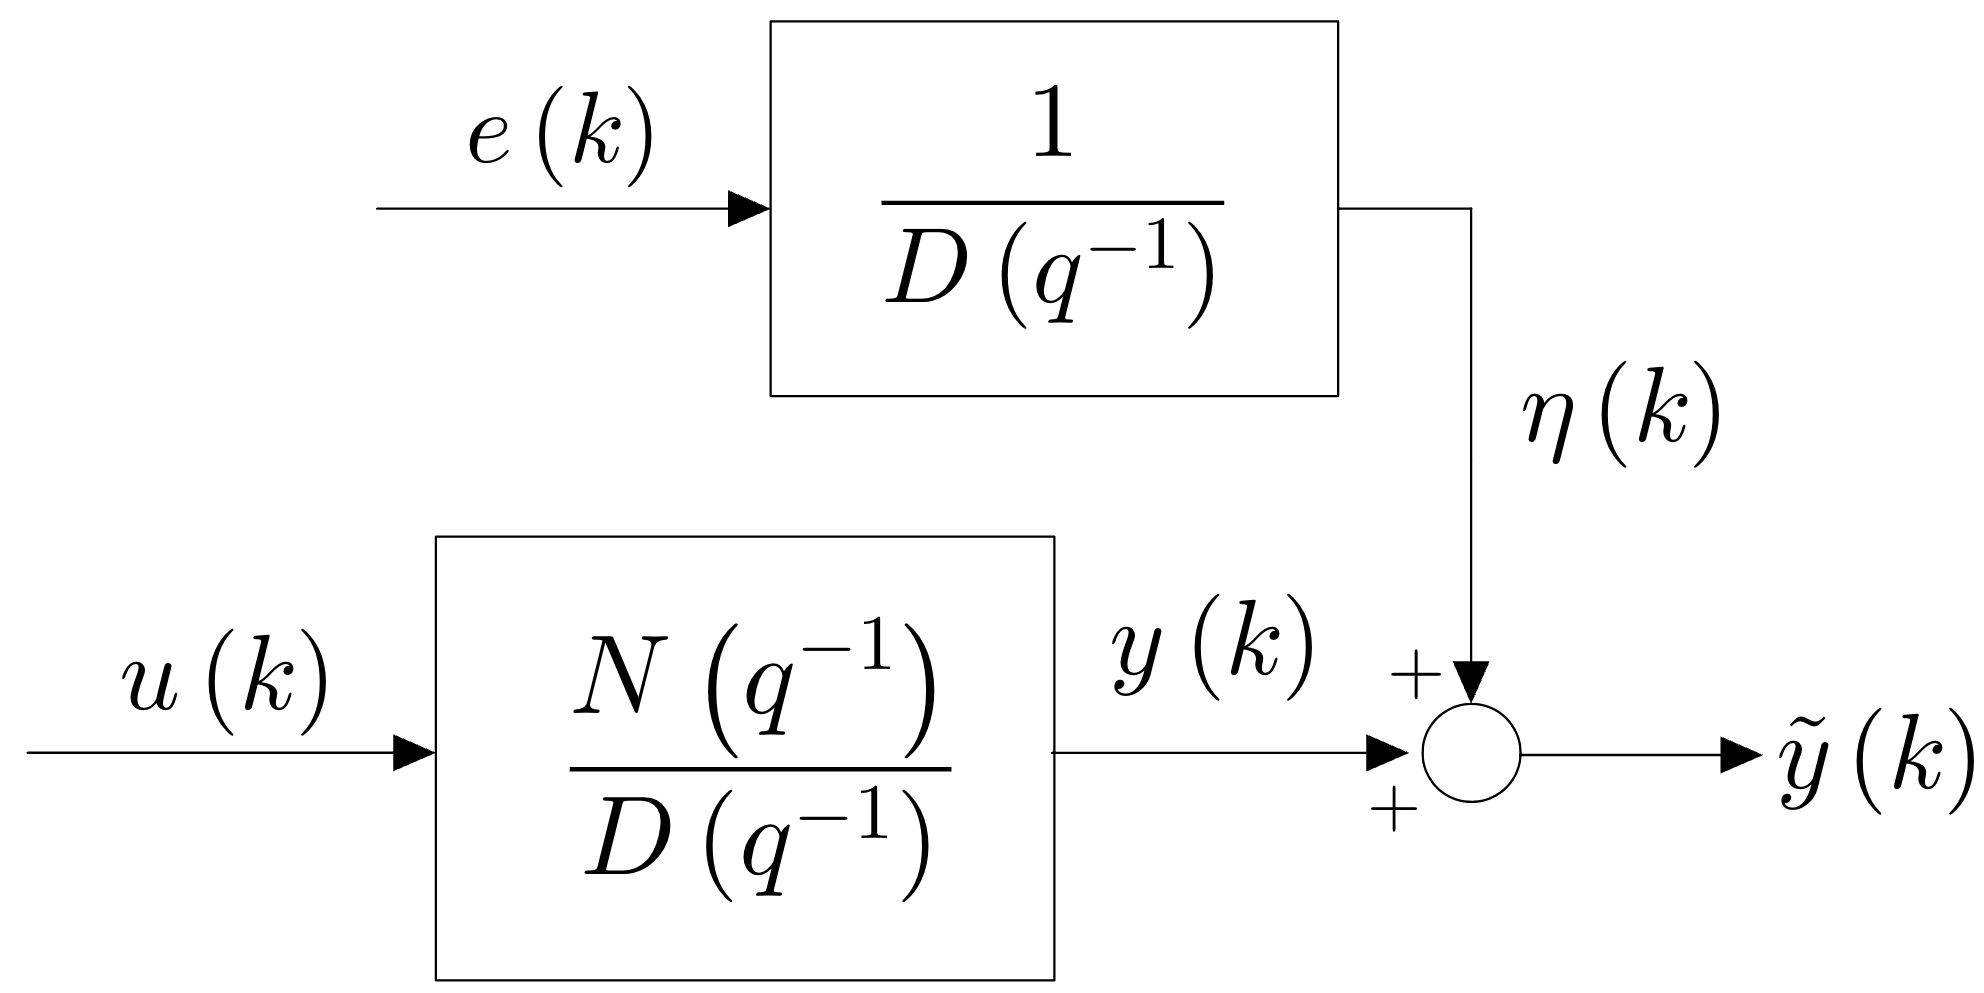
\includegraphics[scale=0.15]{img/EE.jpeg}
    \caption{Equation Error (EE) noise structure}
\end{figure}

\noindent
In this way we can conclude that the LS estimate makes sense if the date corrupted by a random sequence $e(k)$ (the noise) filtered by a system whose transfer function is the denominator of the system to be identified! No sense, since the sensor in general has nothing to share with the plant we want to identify. 
However there are some cases in which the LS approach can be used, we refer to the few cases in which the plant to be identified is such that $D(q^{-1})=1$. This occurs when I have to do:
\begin{itemize}
    \itemsep-0.2em
    \item Identification of \textbf{FIR systems} (Finite impulse response); 
    \item Identification of static systems;
\end{itemize}
\noindent
When the denominator of the transfer function is equal to one, the Equation Error plays the role of the \textit{output measurement error} $\eta(k)$. In this case also the \textbf{second assumption} is satisfied.


\subsection{System Identification of Finite Impulse Response (FIR) systems}
This of type of system has a transfer function which depends only on the samples of the input and not on on the previous output samples.

\begin{equation}
    \tilde{y}(k)=\theta_1{u(k)}+\theta_2{u(k-1)}+...+\theta_n{u(k-n)}+
    \underbrace{e(k)}_{\eta(k)}
\end{equation}
Here also the second assumption is satisfied since the error samples are iid. In the case of FIR the property (\ref{eq:consistency}) is fulfilled.

\subsection{System Identification of Static systems}
Here the output is a function of parameters $\theta_i$ and of the input $u(k)$ at the current instant.
\begin{equation}
    y(k)=\theta_1{g_1({u(k)})} + 
    \theta_2{g_2({u(k)})} + ... +
    \theta_n{g_n({u(k)})} + e(k)
\end{equation}
The functions $g_i(u(k))$ can be trigonometric functions, polynomial or anyway any other basic function.\\

\hrule
\begin{center}
    \textsf{
        Beyond the $\ell_2$ (Least-Squares) estimator, there are other estimators that under the assumption for the noise of satisfying some statistichal properties, are consistent ones. The \textbf{consistency} deals with the property for the expected value of an estimator to converge to the real value $\theta$ of the parameter vector with the increasing number of data. In the following the $\ell_\infty$-norm and $\ell_1$-norm estimators are presented with their features. Moreover a transformation of such problems into Linear Programs is sketched.
    }
\end{center}
\section{$\ell_\infty$-norm parameter estimation}
The $\ell_\infty$-norm parameter estimation is issued by properly solving the following optimization problem: 
{\large{
    \color{red}
    \begin{equation}\label{eq:linfty}
        \theta_{\ell_\infty} = \arg\min_{\theta\in\mathbb{R}^p} {\Vert y-A\theta\Vert_\infty} 
    \end{equation}
}}

It can be demonstrated that under the assumption that the uncertainty enters into the identification problem as an \textit{equation error} and $e(k)\sim{U([-a,a])}$\footnote{
    Uniform probability distribution
}, the estimator in (\ref{eq:linfty}) is consistent. This is equivalent to say:
\begin{equation*}
    \lim_{N\to\infty} {\mathbb{E}[\theta_{\ell_\infty}]}=\theta
\end{equation*}
It is remarkable that using the \textbf{epigraphic formulation} in (\ref{eq:linfty}) the following problem can be recasted into a \textbf{Linear Program} (LP). In particular, keeping in mind that
\begin{equation*}
    \Vert y-A\theta \Vert_\infty \doteq \max_i {\vert y_i-a_i^T\theta \vert}
\end{equation*}
the problem can be rewritten, introducing a \textbf{scalar slack variable} $t$ and pushing the objective in the constraints\footnote{
    Note that: $\max_i {\vert y_i-a_i^T\theta \vert} \le t \iff\vert y_i-a_i^T\theta \vert \le t \quad \forall i $
}:
\begin{equation}
    \begin{aligned}
        &\min_{\theta\in\mathbb{R}^p, t\in\mathbb{R}} t\\
        &\text{s.t.} \ 
         \vert y_i-a_i^T\theta \vert \le t \quad \forall i 
    \end{aligned}
\end{equation} 
An \textit{augmented optimization variable} $x=[\theta, t]\in\mathbb{R}^{p+1}$ can be used in order to transform the original problem into: 
\begin{equation}\label{eq:LP_prob}
    \begin{aligned}
        &\min_{x} c^T{x}\\
        &\text{s.t.} \ \tilde{A}\theta\le{\tilde{b}}
    \end{aligned}
\end{equation}
where 
\begin{equation}
    \tilde{A}=\begin{bmatrix}
        -A&-\mathbf{1}\\
        A&\mathbf{-1}
    \end{bmatrix}, \quad
    \mathbf{1} = [1\ 1 \ ... \ 1]^T, \quad
    \tilde{b}=\begin{bmatrix}
        -y\\
        y
    \end{bmatrix}
\end{equation}

\section{$\ell_1$-norm parameter estimation}
The $\ell_1$-norm parameter estimation is performed by solving the following optimization problem: 
{\large{
    \color{red}
    \begin{equation}\label{eq:lone}
        \theta_{\ell_1} = \arg\min_{\theta\in\mathbb{R}^p} \Vert y-A\theta \Vert_1 = \arg \min_{\theta\in\mathbb{R}^p} \sum_{i=1}^m \vert y_i-a_i^T\theta \vert 
    \end{equation}
}}
In a similar way we have seen for the $\ell_2$ and $\ell_1$ estimators, can be demonstrated that under the assumption of the uncertainty entering the problem as an equation error and the noise samples $e(k)\sim\mathcal{L}(\mu,b)$\footnote{
    Laplacian probability distribution
}, the $\ell_1$-norm estimator is consistent, in the sense that
\begin{equation}
    \lim_{N\to\infty} \mathbb{E}[\theta_{\ell_1}]=\theta
\end{equation}
Also in this case the problem (\ref{eq:lone}) can be recasted as an LP one, introducing some additional slack variables $t_i$ for each one of the terms of the terms in the summation:
\begin{equation}
    \begin{aligned}
        &\min_{\theta\in\mathbb{R}^p,t\in\mathbb{R}^m} \sum_{i=1}^m t_i\\
        &\text{s.t.} \ 
        \vert y_i-a_i^T\theta \vert \le t_i  \quad i=1,..., m
    \end{aligned}
\end{equation}
Defining $x=[\theta,t]\in\mathbb{R}^{p+m}$ as the augmented optimization variable, the standard form of a \textit{Linear Program} defined as in (\ref{eq:LP_prob}), by putting:
\begin{equation}
    \tilde{A}=\begin{bmatrix}
        -A&-I\\
        -A&I
    \end{bmatrix}, \ b=\begin{bmatrix}
        -y\\
        y
    \end{bmatrix}
\end{equation}
where $I$ is the identity matrix $m\times{m}$.

\section{Final remarks}
Real experimets have data characterized by noise and in general the consistency property does not hold, in some situations in which the problem has a particular structure the assumptions required are perfectly fulfilled. We have understood that the most critical problem to manage is the second assumption which require the error to be white, zero mean and Gaussian (very strong assumptions!), moreover the resulting noise structure reaches a quite strange conclusion in which it is required that the system and the sensor share a part of their model. \\
In the following we will see another approach that, differently from LS, replaces the Assumption (2) with something that is significantly \textit{less strong}.

